\chapter{Experiment}

\section{Overview}

\begin{minipage}{0.33\textwidth}
    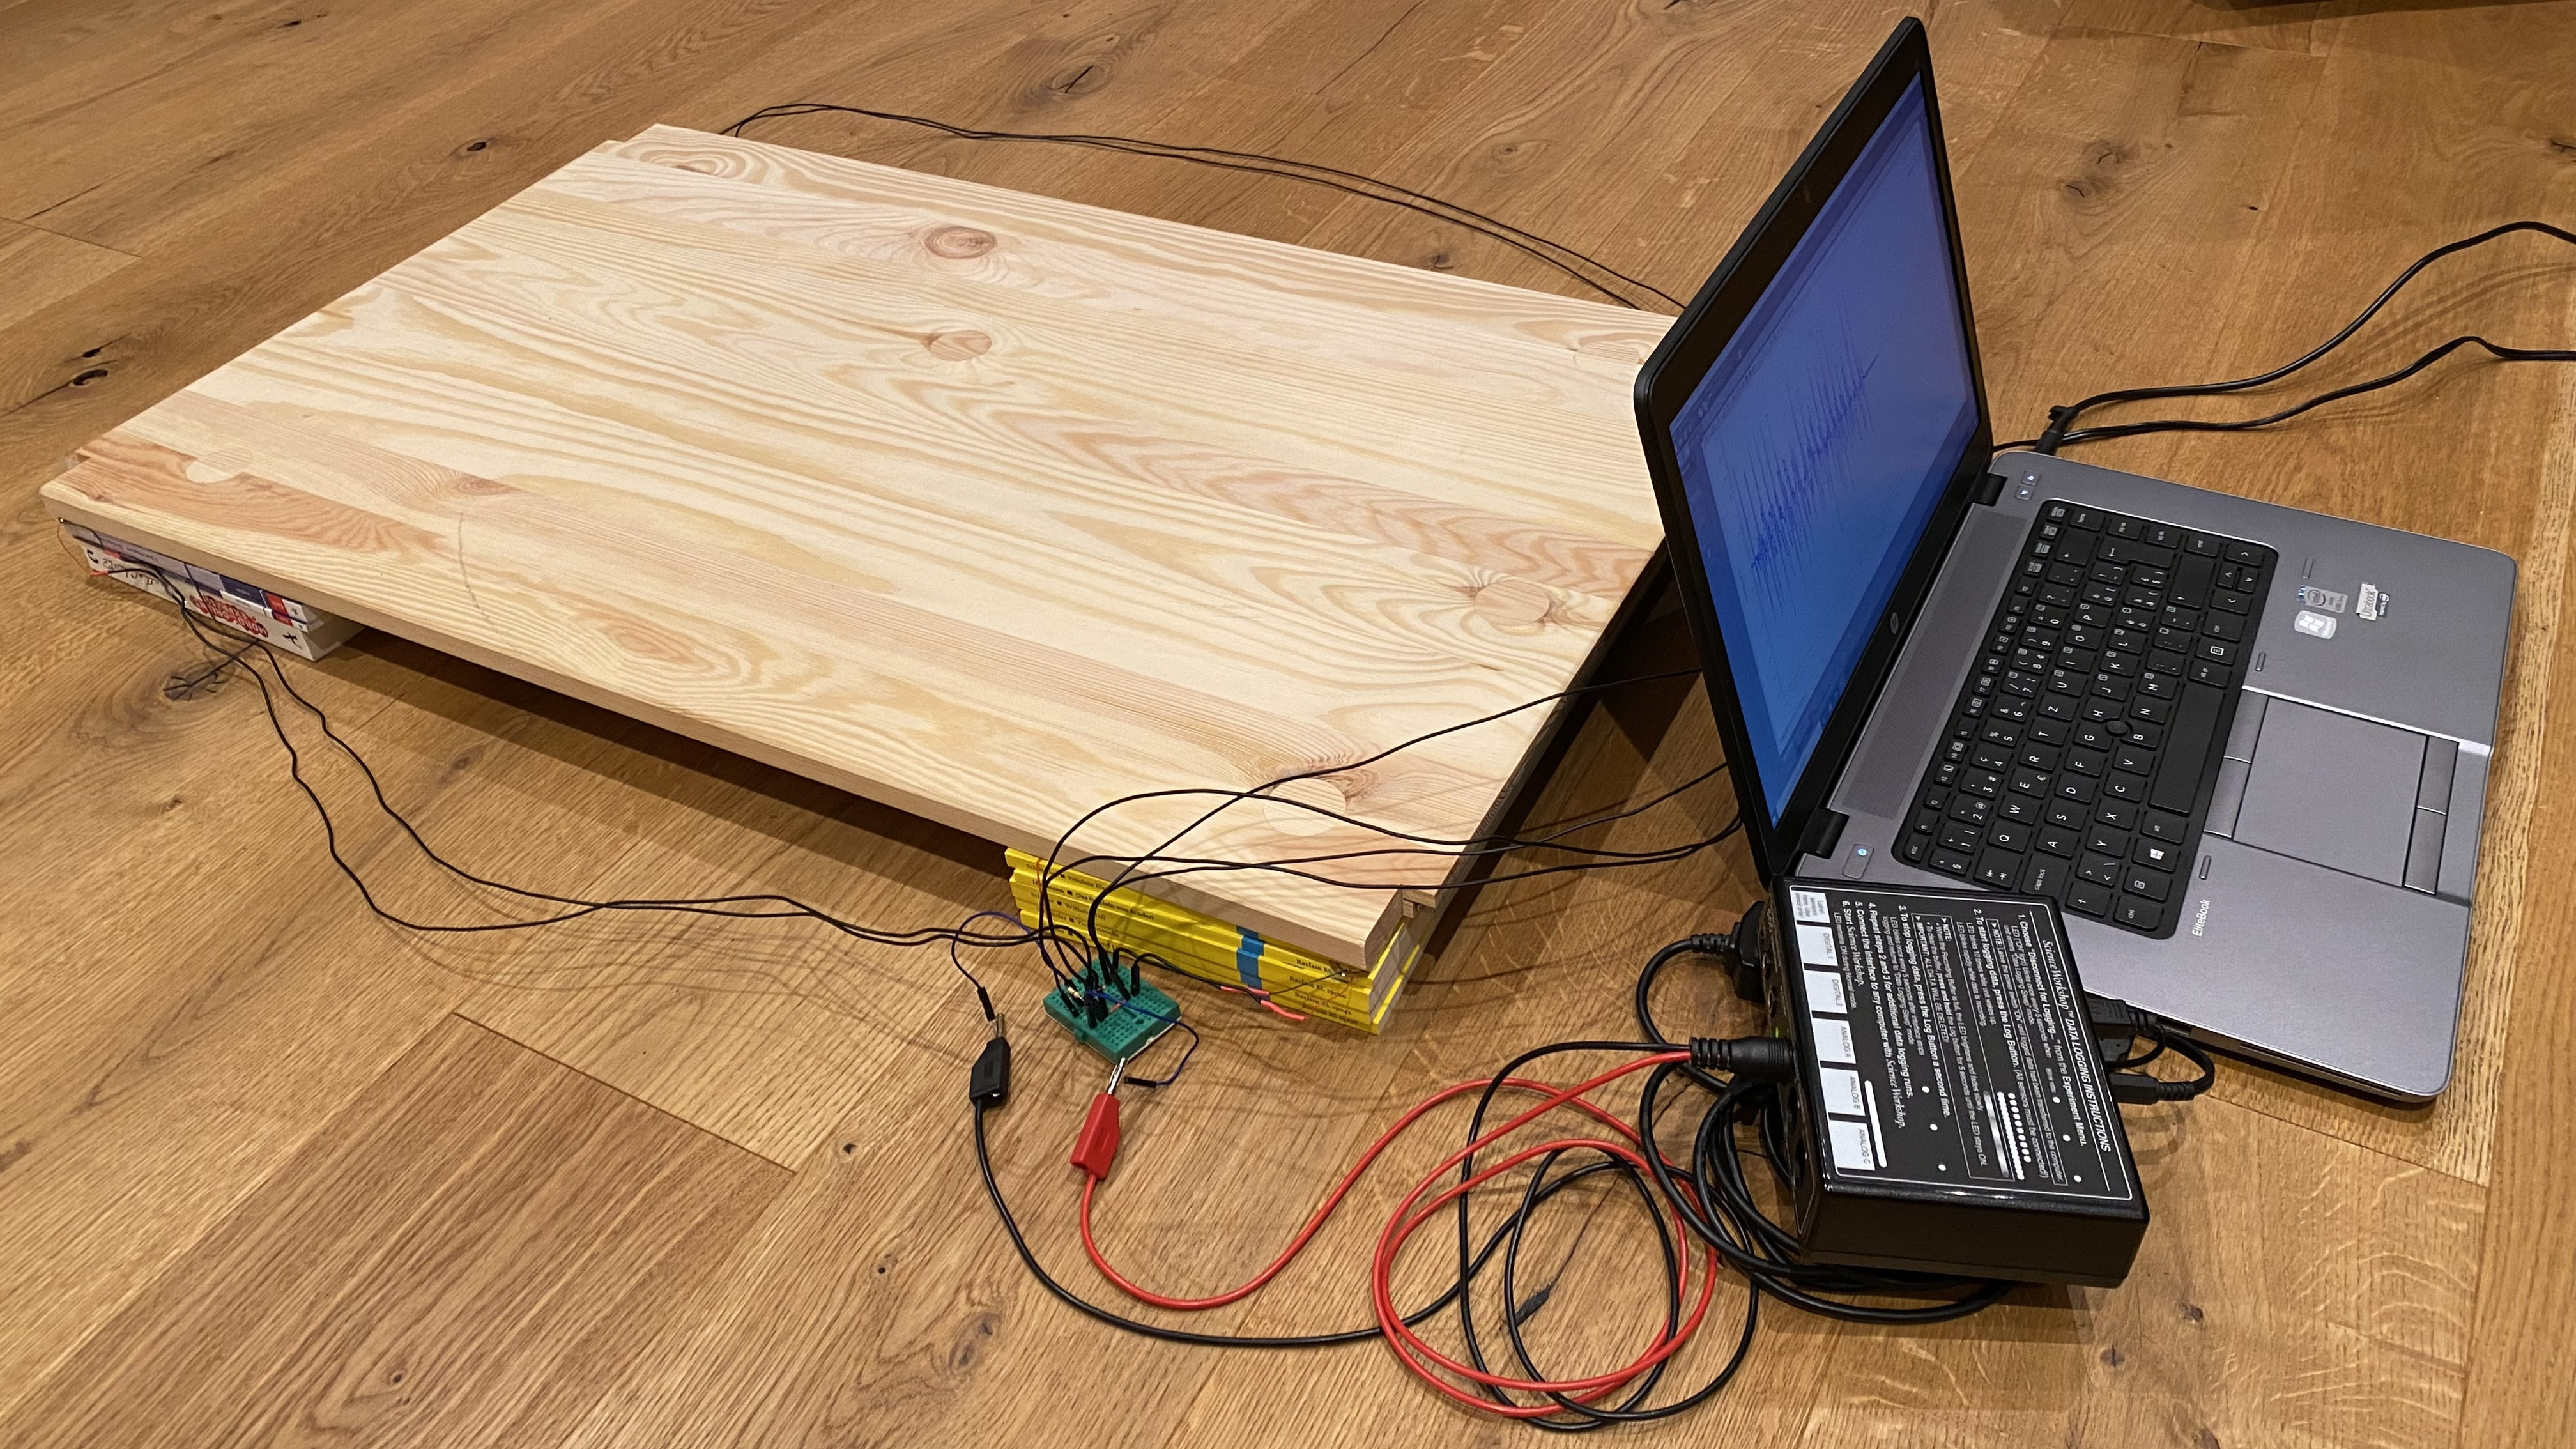
\includegraphics[width=\textwidth]{./Figure_6.jpg}
    \captionof{figure}{Experiment}
    \label{fig:Experiment}
\end{minipage}
\begin{minipage}{0.66\textwidth}
    For the experiment four piezoelectric elements were placed under the corners of a wooden board of dimensions $0.8 \times 0.4 \times 0.02$ m. These were then connected to a brad board parallel to a $470k\Omega$ resistor. A voltmeter was connected to the resistor and measured the voltage output while a person was jumping on the wooden board from a height of 20 cm $\pm 1$ cm.\\
\end{minipage}
\begin{minipage}{0.33\textwidth}
    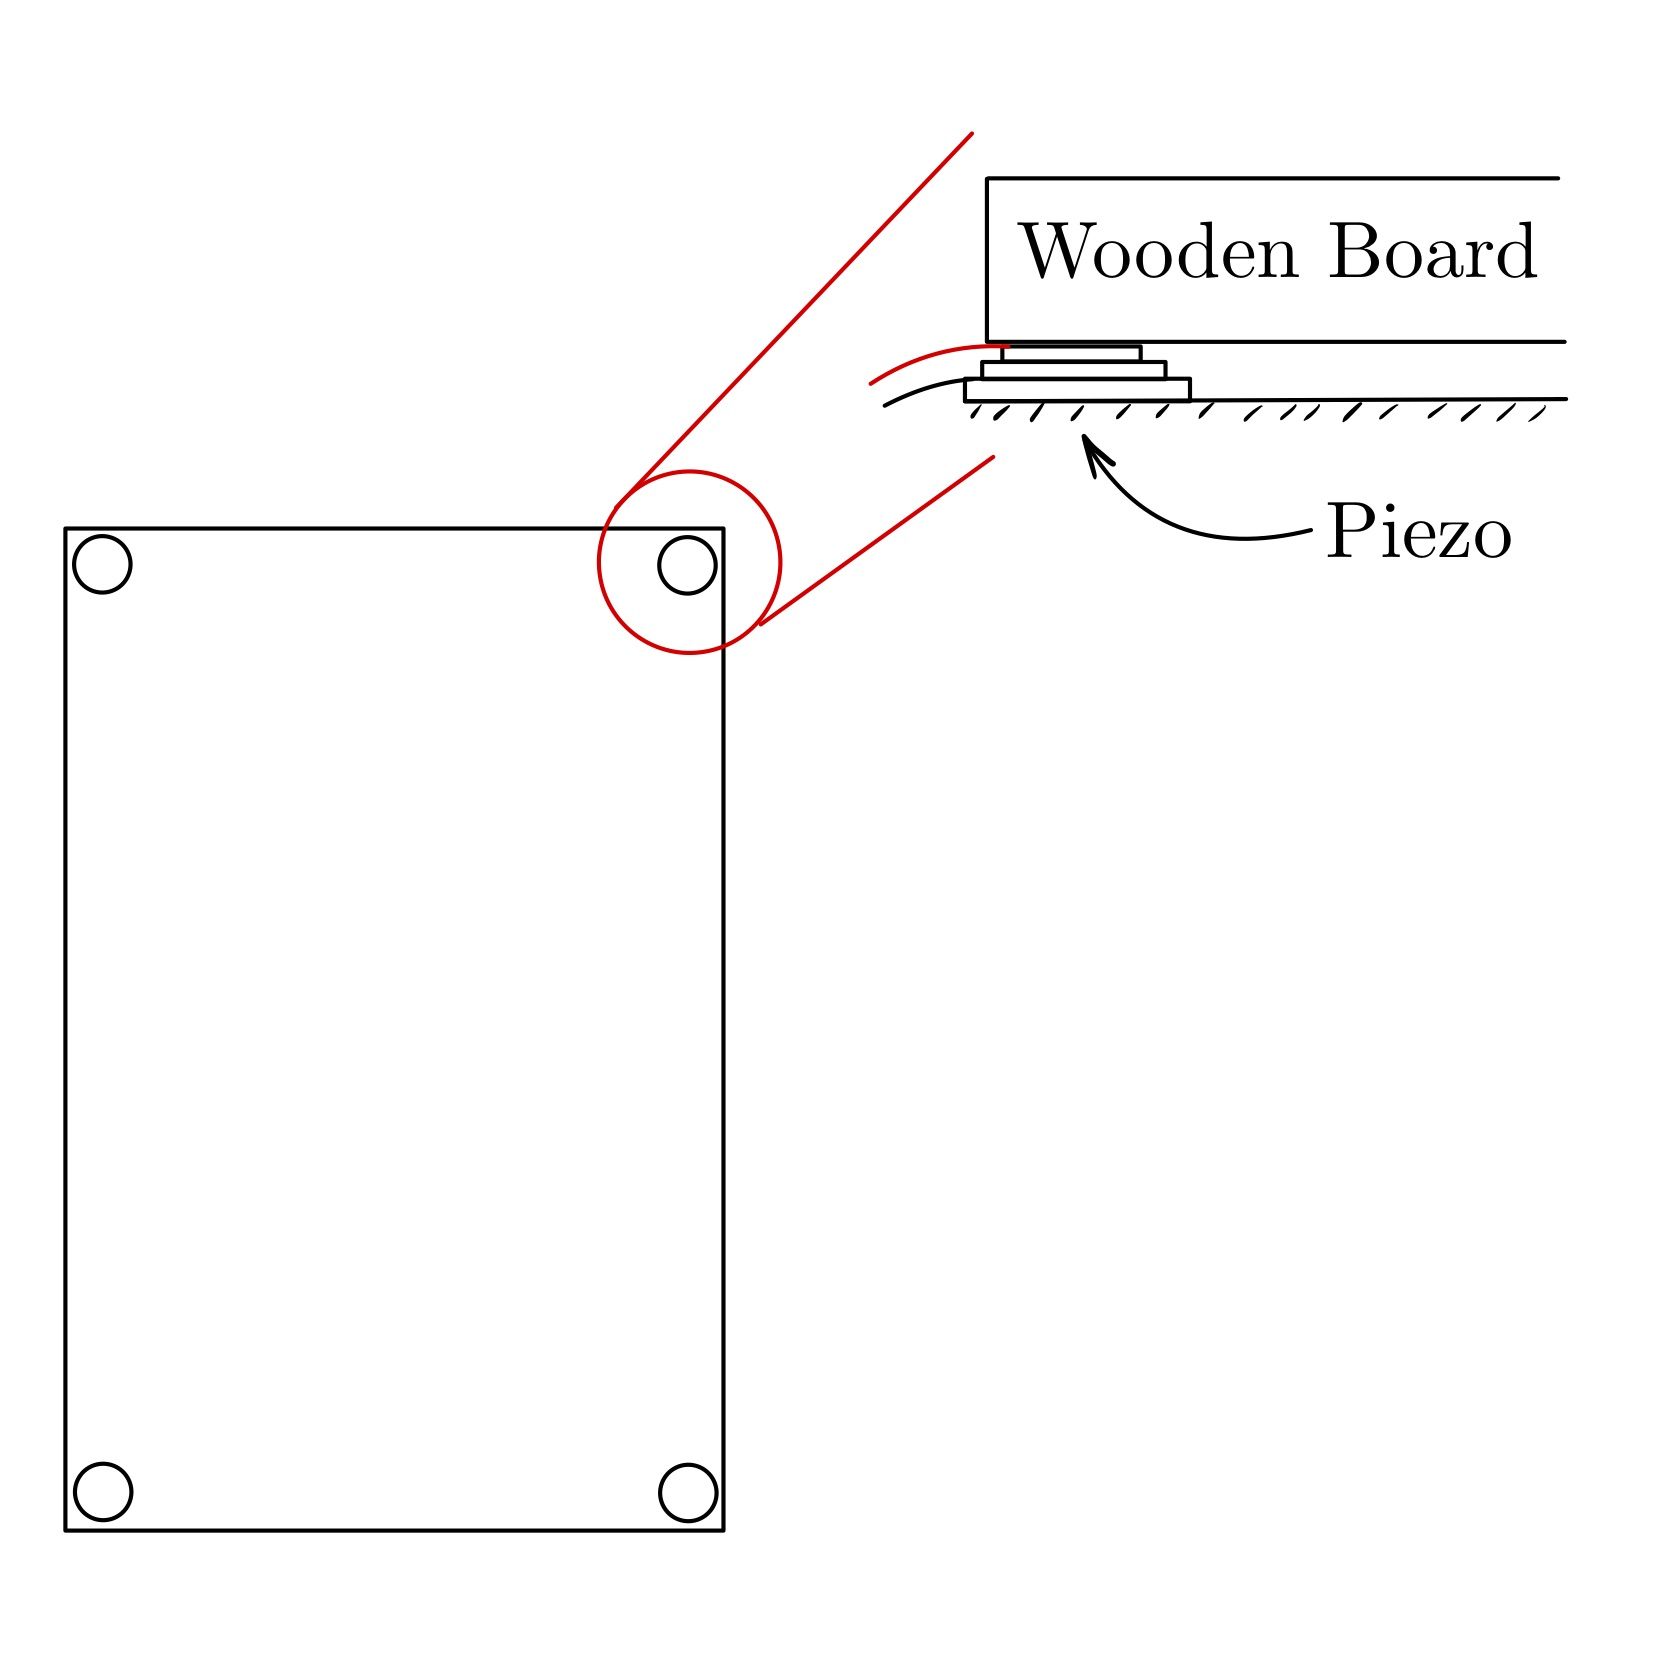
\includegraphics[width=\textwidth]{./Figure_7.jpg}
    \captionof{figure}{Wooden board with piezoelectric elements}
    \label{fig:Wooden board with piezoelectric elements}
\end{minipage}
\begin{minipage}{0.66\textwidth}
    To get an ideal result, the board must be elevated. This ensures an ideal result for the experiment since all the force will be applied onto the four piezo electric elements.\\
\end{minipage}
\begin{minipage}{0.33\textwidth}
    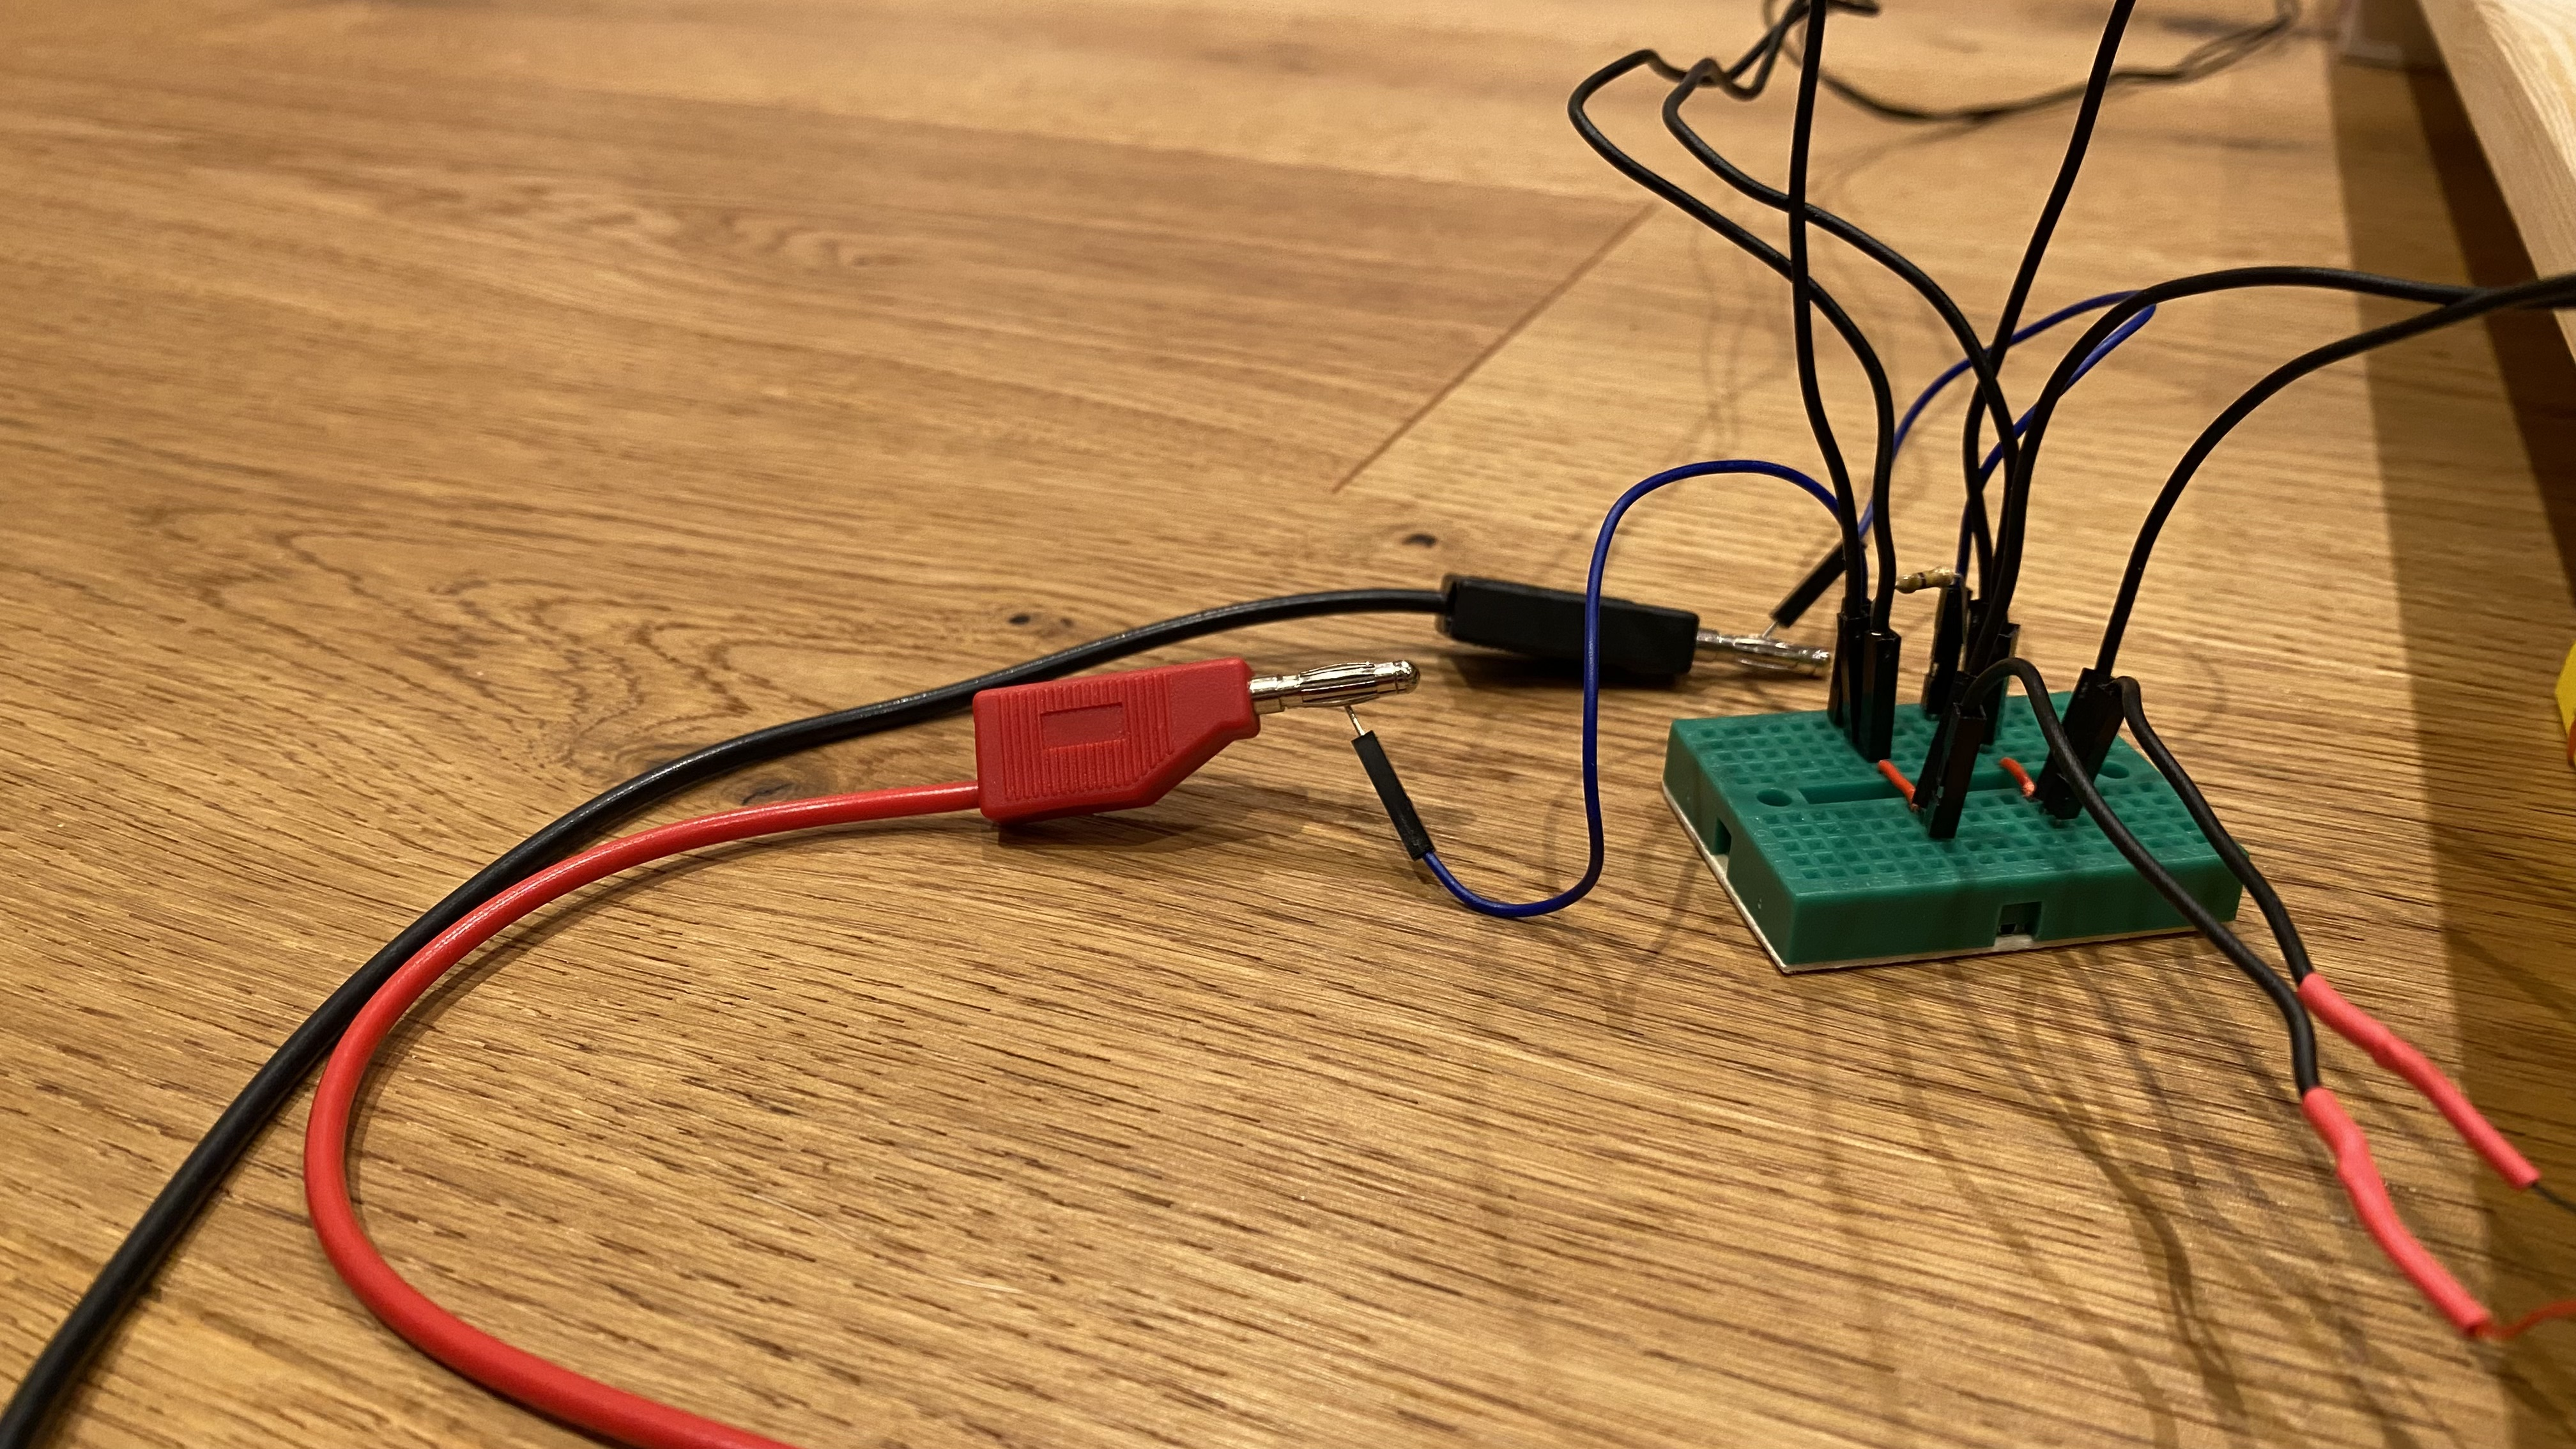
\includegraphics[width=\textwidth]{./Figure_8.jpg}
    \captionof{figure}{Piezoelectric Elements connected in parallel}
    \label{fig:Piezoelectric Elements connected in parallel}
\end{minipage}
\begin{minipage}{0.33\textwidth}
    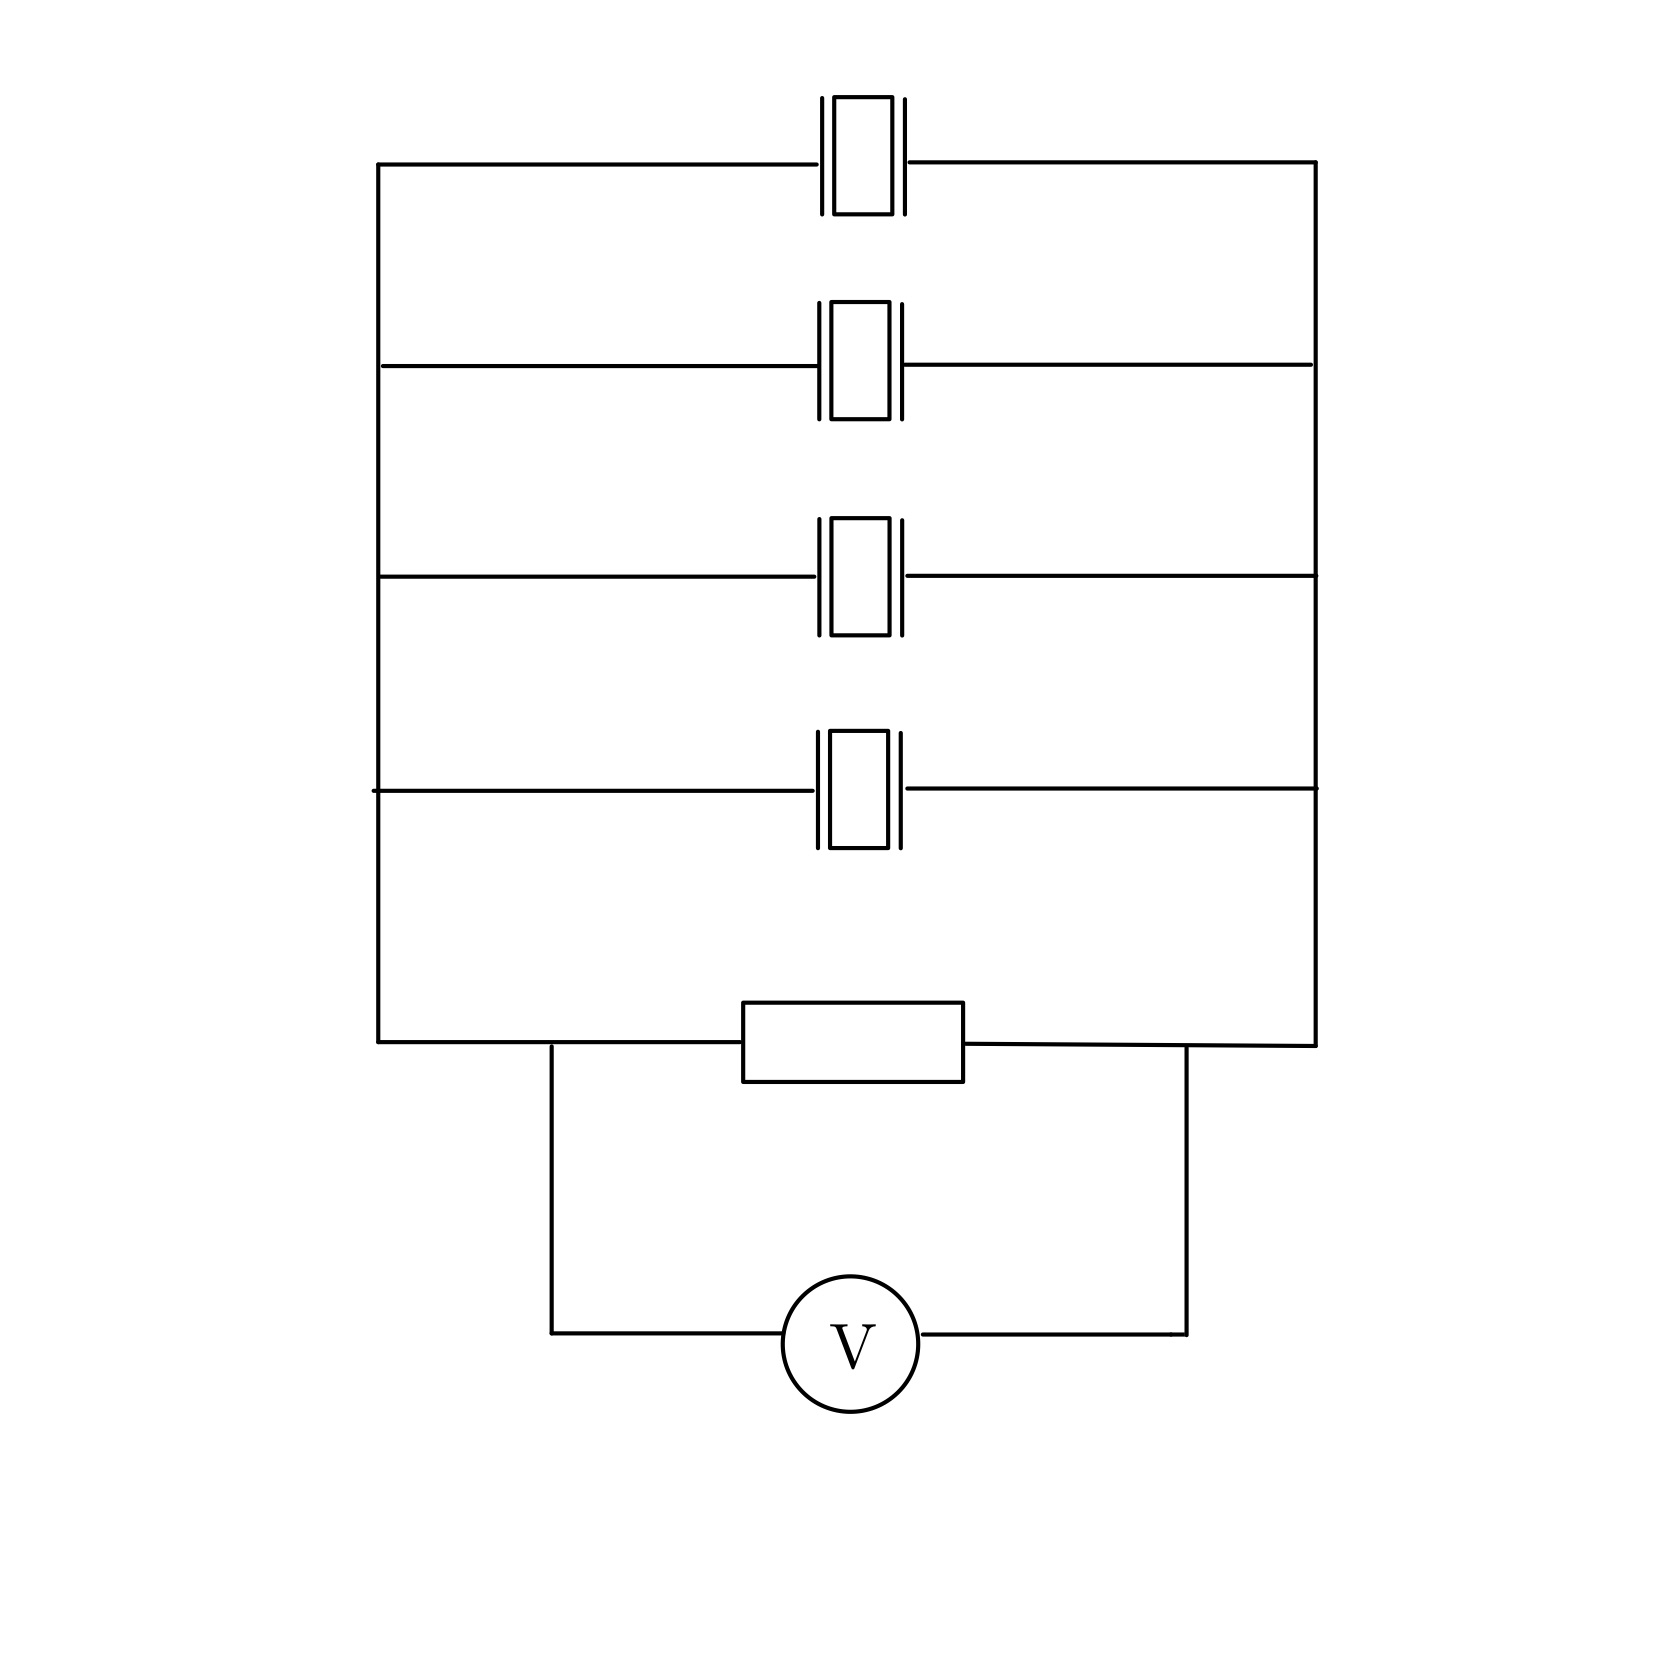
\includegraphics[width=\textwidth]{./Figure_9.jpg}
    \captionof{figure}{Circuit Diagram}
    \label{fig:Circuit Diagram}
\end{minipage}
\begin{minipage}{0.33\textwidth}
    The piezoelectric elements were connected in parallel in addition with a $470k\Omega$ resistor. As represented in Figure \ref{fig:Piezoelectric Elements connected in parallel} the voltmeter was then parallel connected to the resistor.\\
\end{minipage}
\begin{minipage}{0.33\textwidth}
    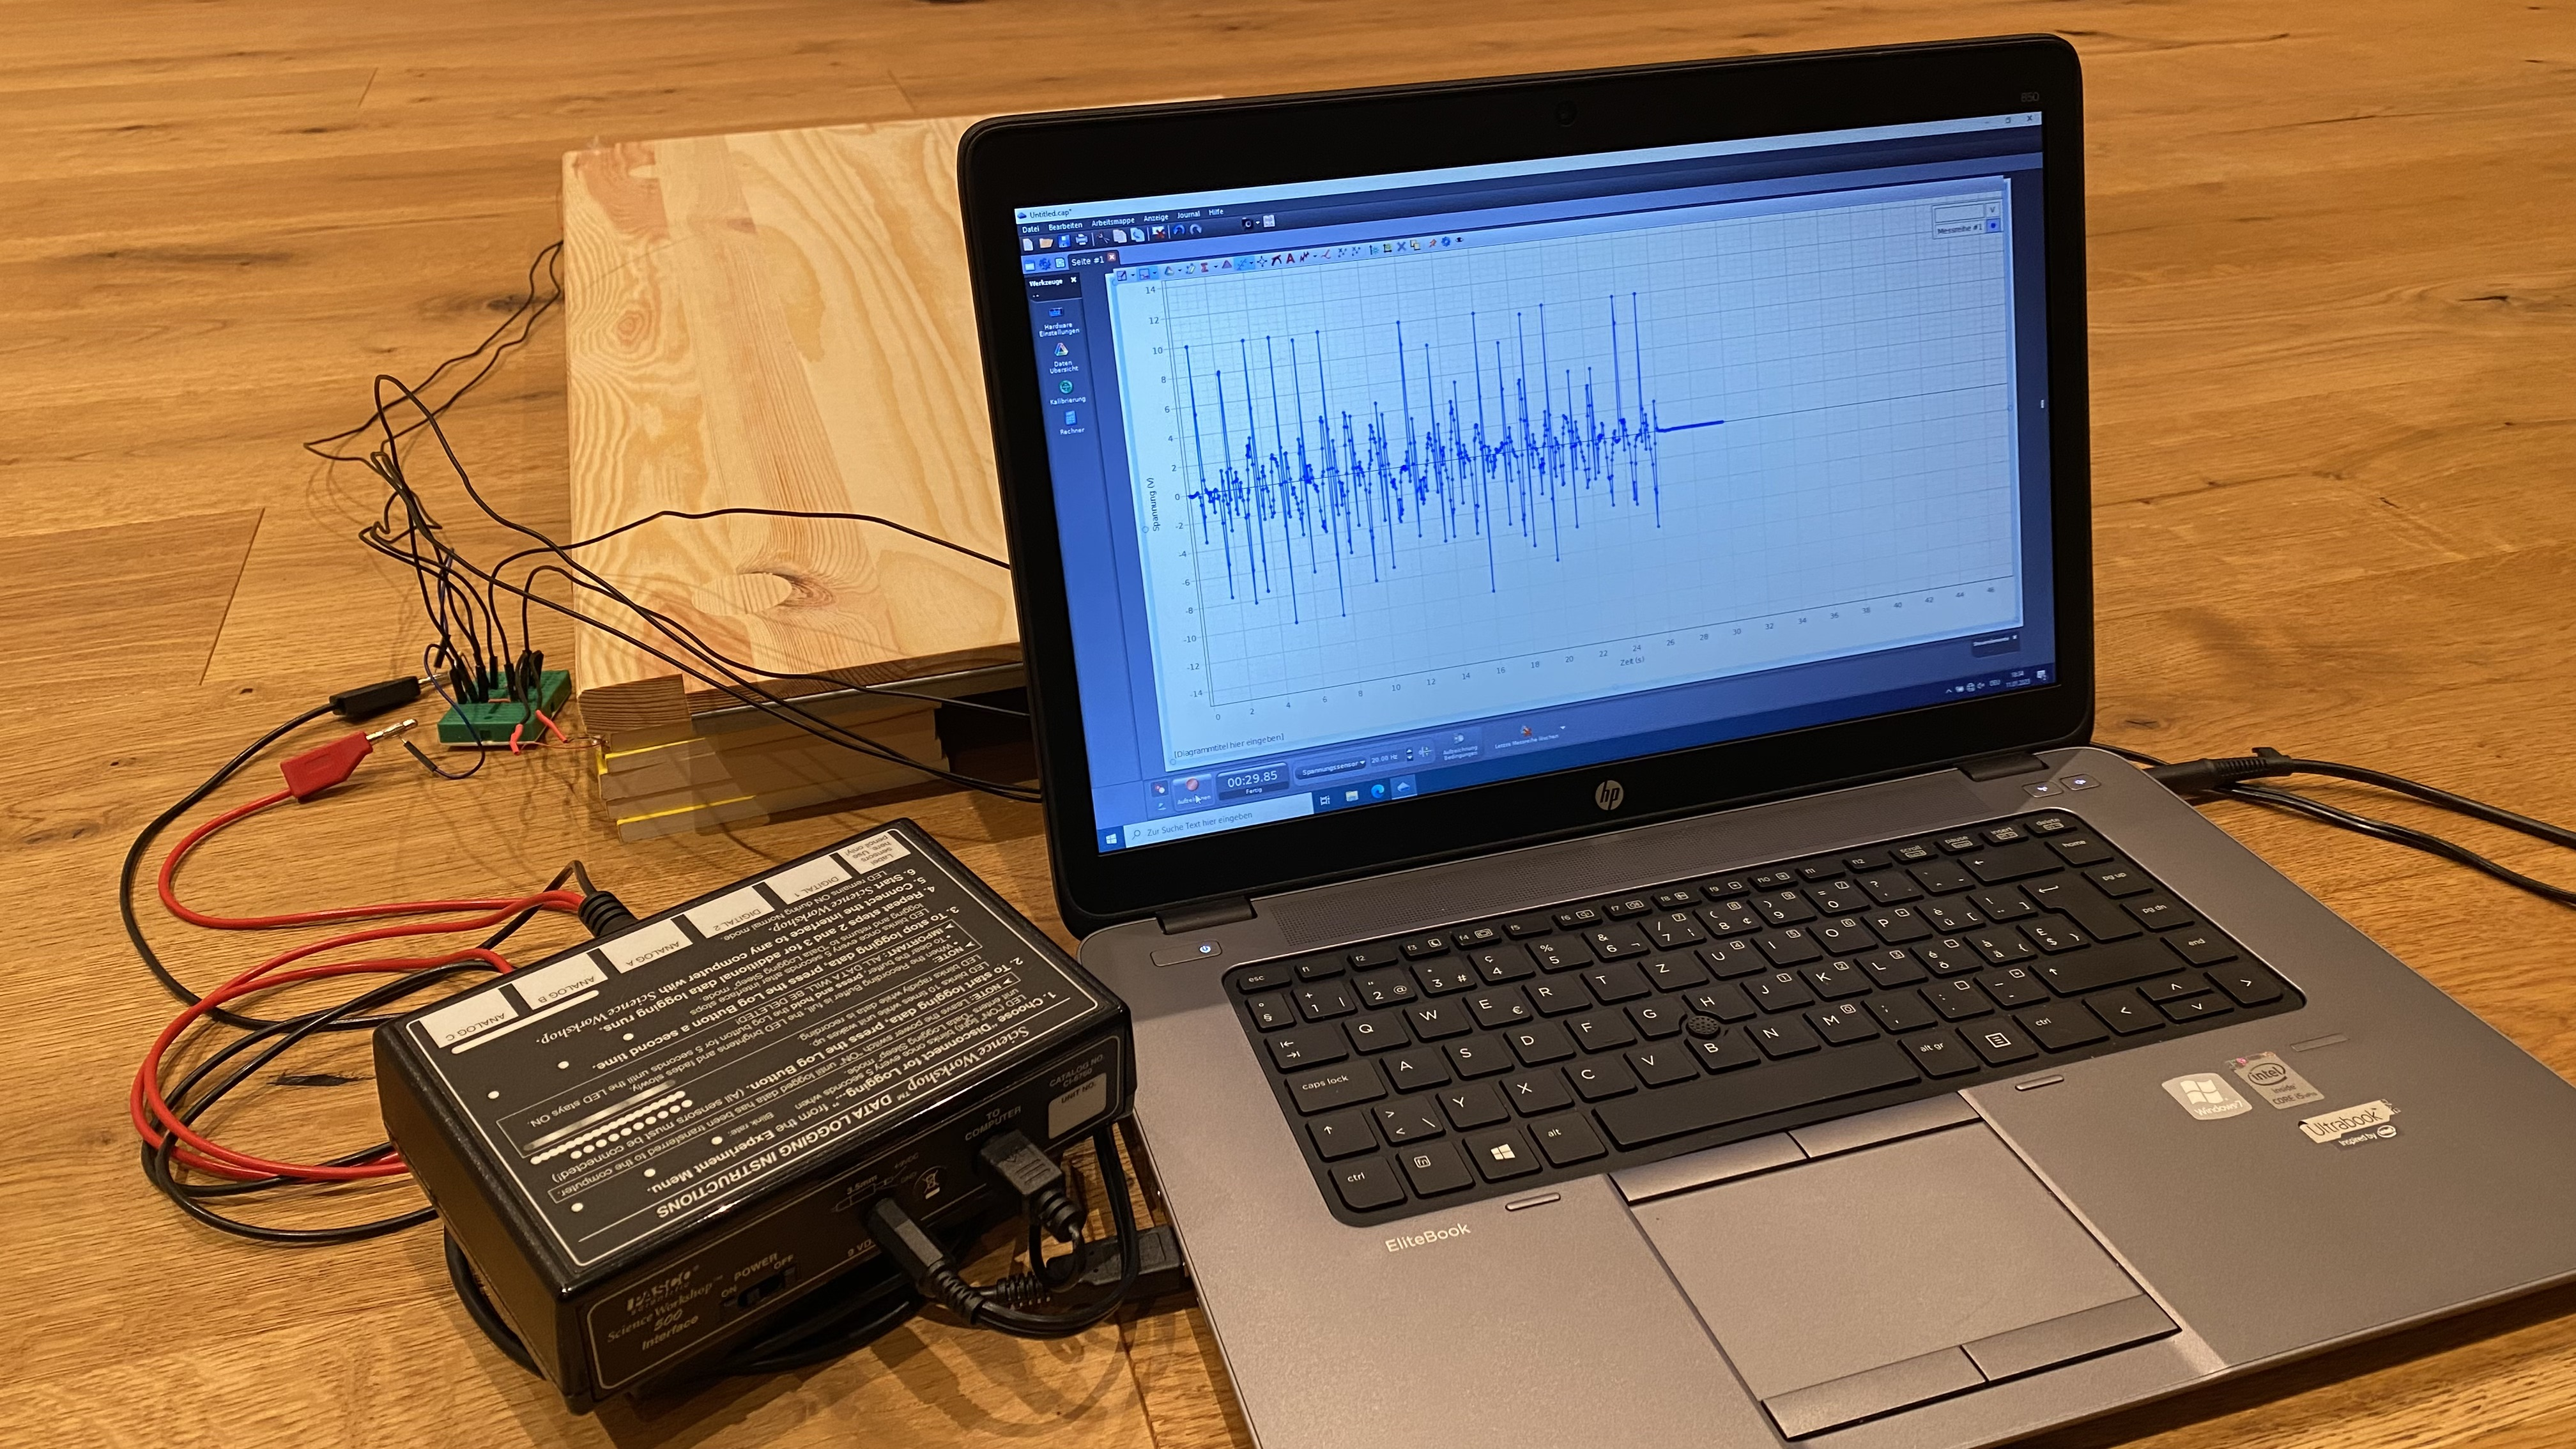
\includegraphics[width=\textwidth]{./Figure_10.jpg}
    \captionof{figure}{Laptop and Pasco Interface 500}
    \label{fig:Laptop and Pasco Interface 500}
\end{minipage}
\begin{minipage}{0.66\textwidth}
    For the measurement, a Pasco 500 Interface was used to measure the voltage. A laptop logged the data and plotted graphs.
\end{minipage}
\subsection{Theoretical Calculation of the Experiment}

The formula $U = g \cdot \frac{F \cdot t}{A}$ can be used to calculate the voltage output of the four piezoelectric elements.The impact force is estimated to be $730 \pm 2$ N. This results in a voltage of $10.81 \pm 0.03$ V. 
$$
U = g \cdot \frac{F \cdot t}{A}
$$
\begin{equation*}
    \begin{split}
    U & = \frac{U_{\text{max}}+ U_{\text{min}}}{2} \pm \frac{U_{\text{max}}- U_{\text{min}}}{2}\\
    & = 10.81 \pm 0.03 V
    \end{split}
\end{equation*}
With the voltage calculated, the formula $P = \frac{U^2}{R}$ can now be used to calculate the predicted power output. Hence, the power output is $249 \pm 14$ $\mu$W.
$$
P = \frac{V^2}{R}
$$
\begin{equation*}
    \begin{split}
        P & = \frac{P_{\text{max}}+ P_{\text{min}}}{2} \pm \frac{P_{\text{max}}- P_{\text{min}}}{2}\\
    & = 249 \pm 14 \mu W
    \end{split}
\end{equation*}

\section{Results}

\begin{minipage}{0.5\textwidth}
    \center
        \begin{tabular}{|c|c|}
        \hline
        Time in s & Voltage in V \\
        \hline
        0 & -0.083 \\
        \hline
        0.05 & 1.353\\
        \hline
        0.1 & 9.995\\
        \hline
        0.15 & -1.562\\
        \hline
        0.2 & 0.459\\
        \hline
        0.25 & 0.781\\
        \hline
        0.3 & 1.646\\
        \hline
        0.35 & 0.908\\
        \hline
        0.4	& 0.068\\
        \hline
        0.45 & -0.156\\
        \hline
        0.5	& -0.596\\
        \hline
        0.55 & -0.19\\
        \hline
        0.6	& 0.234\\
        \hline
        0.65 & 0.205\\
        \hline
        0.7	& 0.122\\
        \hline
        0.75 & -0.029\\
        \hline
        0.8	& 0.049\\
        \hline
        0.85 & 0.098\\
        \hline
        0.9	& 0.044\\
        \hline
        \end{tabular}
        \captionof{table}{Values of Voltage Graph 1}
        \label{Tab:Values of Voltage Graph 1}
\end{minipage}
\begin{minipage}{0.5\textwidth}
    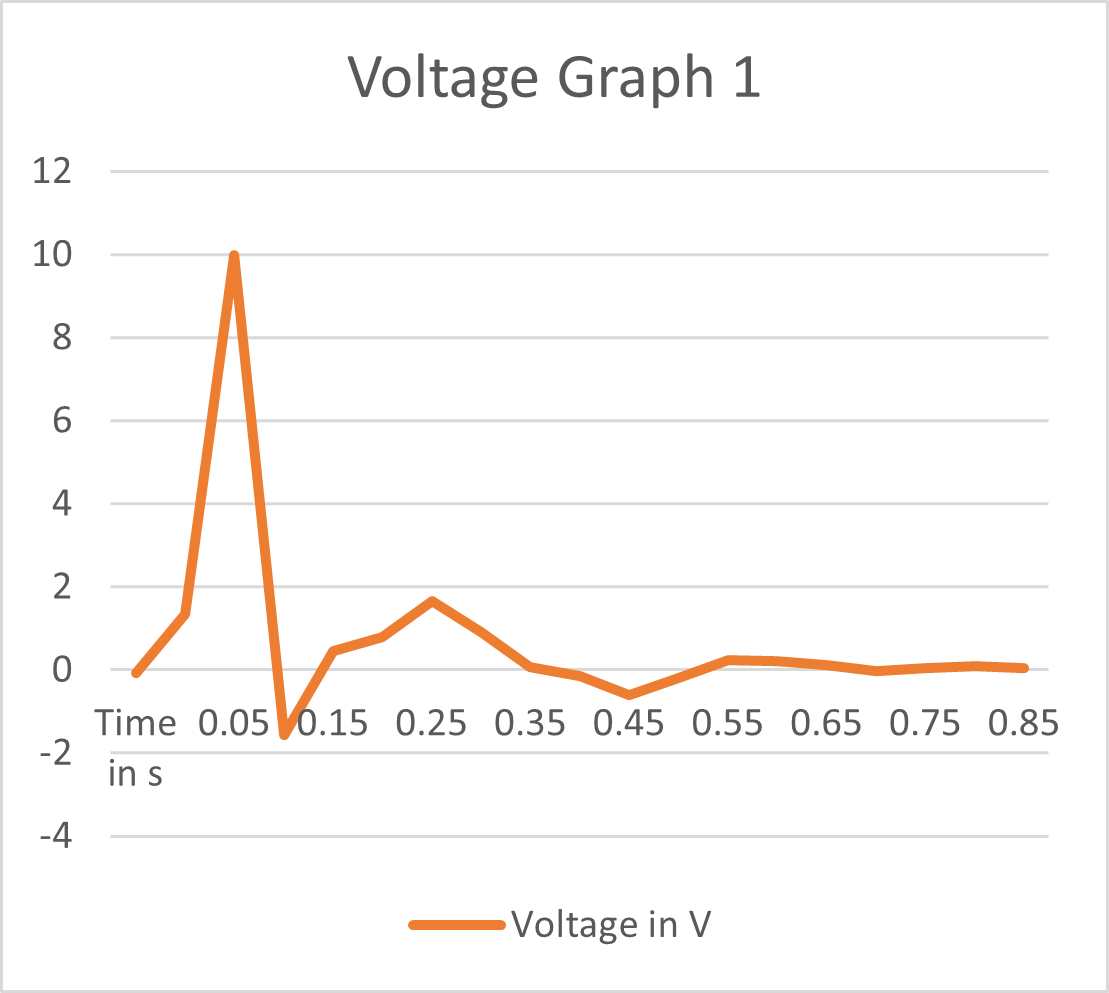
\includegraphics[width=\textwidth]{./Figure_11.png}
    \captionof{figure}{Voltage Graph 1}
    \label{fig:Voltage Graph 1}
\end{minipage}
\newpage
\begin{minipage}{0.5\textwidth}
    \center
        \begin{tabular}{|c|c|}
            \hline
            Time in s & Voltage in V \\
            \hline
            0 & -0.151\\
            \hline
            0.05 & -0.107\\
            \hline
            0.1	& -0.088\\
            \hline
            0.15 & -2.334\\
            \hline
            0.2	& 9.995\\
            \hline
            0.25 & -1.401\\
            \hline
            0.3	& -0.137\\
            \hline
            0.35 & 0.181\\
            \hline
            0.4 & 0.723\\
            \hline
            0.45 & 1.533\\
            \hline
            0.5	& 1.86\\
            \hline
            0.55 & 1.24\\
            \hline
            0.6	& 0.415\\
            \hline
            0.65 & -0.02\\
            \hline
            0.7	& -0.063\\
            \hline
            0.75 & -0.273\\
            \hline
            0.8	& 0.249\\
            \hline
            0.85 & 0.195\\
            \hline
            0.9	& -0.156\\
            \hline
            0.95 & -0.054\\
            \hline
            1 & 0.088\\
            \hline
            1.05 & 0.166\\
            \hline
            1.1	& 0.132\\
            \hline
            1.15 & 0.215\\
            \hline
            1.2	& 0.093\\
            \hline
        \end{tabular}
        \captionof{table}{Values of Voltage Graph 2}
        \label{Tab:Values of Voltage Graph 2}
\end{minipage}
\begin{minipage}{0.5\textwidth}
    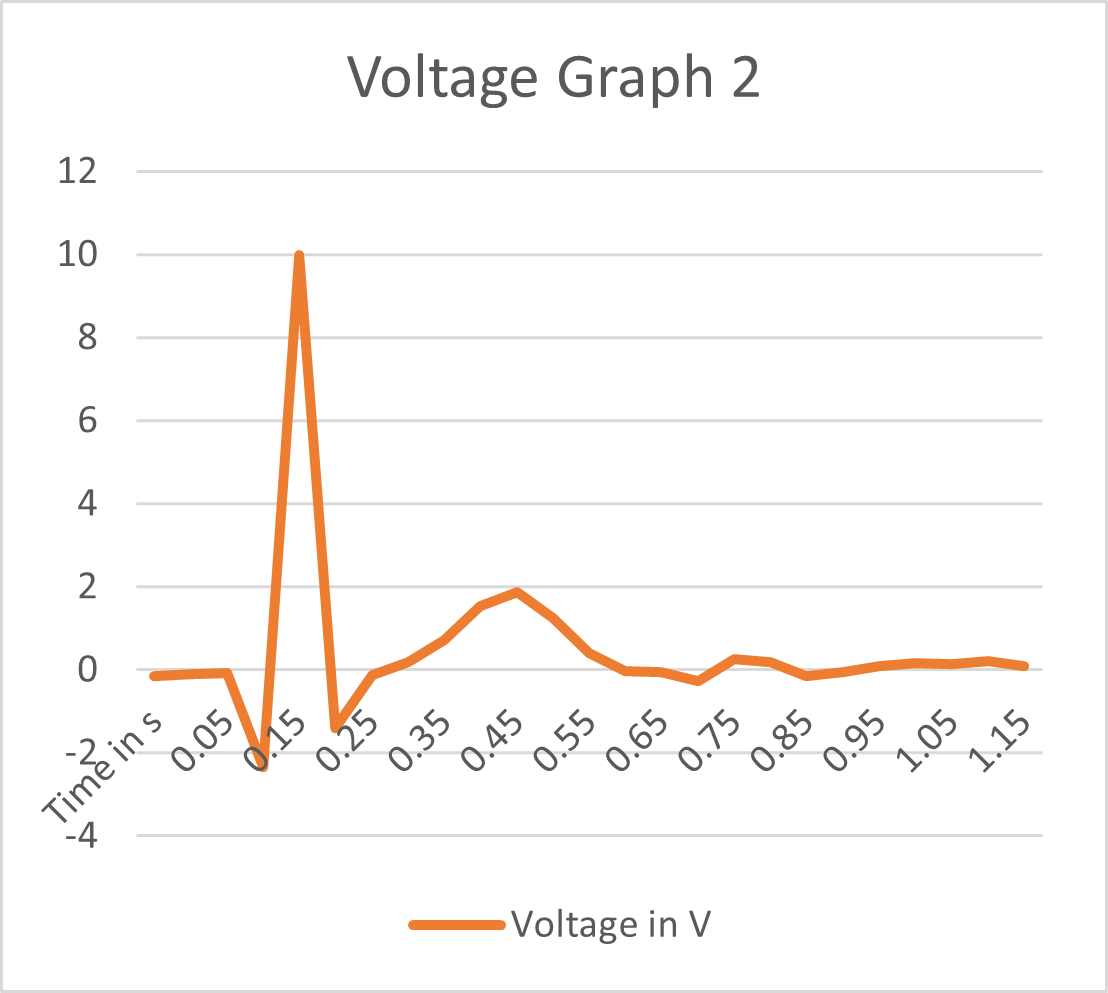
\includegraphics[width=\textwidth]{./Figure_12.png}
    \captionof{figure}{Voltage Graph 2}
    \label{fig:Voltage Graph 2}
\end{minipage}

\newpage

\begin{minipage}{0.5\textwidth}
    \center
        \begin{tabular}{|c|c|}
            \hline
            Voltage in V & Time in s \\
            \hline
            0 & 0.283\\
            \hline
            0.05 & 4.844\\
            \hline
            0.1	& -4.932\\
            \hline
            0.15 & -4.673\\
            \hline
            0.2	& -2.393\\
            \hline
            0.25 & -1.045\\
            \hline
            0.3	& -0.479\\
            \hline
            0.35 & -0.259\\
            \hline
            0.4	& -0.171\\
            \hline
            0.45 & -0.122\\
            \hline
            0.5	& -0.098\\
            \hline
            0.55 & -1.826\\
            \hline
            0.6	& 9.995\\
            \hline
            0.65 & -2.822\\
            \hline
            0.7	& 0.591\\
            \hline
            0.75 & 0.19\\
            \hline
            0.8	& 0.62\\
            \hline
            0.85 & 1.143\\
            \hline
            0.9	& 1.396\\
            \hline
            0.95 & 0.869\\
            \hline
            1 & -0.034\\
            \hline
            1.05 & 0.122\\
            \hline
            1.1	& -0.088\\
            \hline
            1.15 & 0.01\\
            \hline
        \end{tabular}
        \captionof{table}{Values of Voltage Graph 3}
        \label{Tab:Values of Voltage Graph 3}
\end{minipage}
\begin{minipage}{0.5\textwidth}
    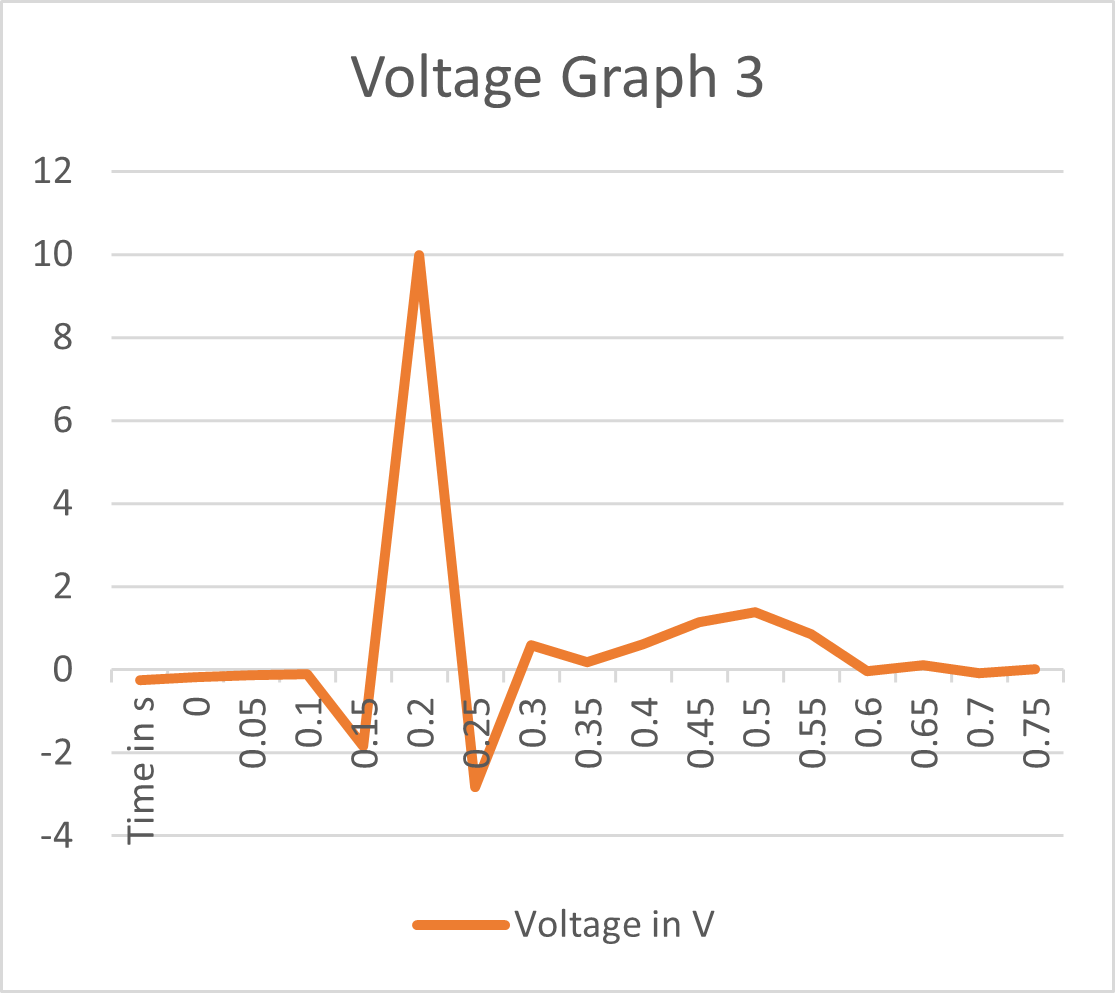
\includegraphics[width=\textwidth]{./Figure_13.png}
    \captionof{figure}{Voltage Graph 3}
    \label{fig:Voltage Graph 3}
\end{minipage}

\vspace{0.5cm}

The table and graphs above show that the voltage output by the piezoelectric elements varies between $-2.822 \pm 0.001$ V and $9.995 \pm 0.001$ V with a discrepancy of $7.54 \pm 2.485 \%$.\\

\begin{minipage}{0.5\textwidth}
    \center
        \begin{tabular}{|c|c|}
            \hline
            Time in s & Power in W \\
            \hline
            0 & 1.46574E-08\\
            \hline
            0.05 & 3.89491E-06\\
            \hline
            0.1	& 0.000212553\\
            \hline
            0.15 & 5.19116E-06\\
            \hline
            0.2	& 4.48257E-07\\
            \hline
            0.25 & 1.29779E-06\\
            \hline
            0.3	& 5.7645E-06\\
            \hline
            0.35 & 1.75418E-06\\
            \hline
            0.4	& 9.8383E-09\\
            \hline
            0.45 & 5.17787E-08\\
            \hline
            0.5	& 7.55779E-07\\
            \hline
            0.55 & 7.68085E-08\\
            \hline
            0.6	& 1.16502E-07\\
            \hline
            0.65 & 8.94149E-08\\
            \hline
            0.7	& .16681E-08\\
            \hline
            0.75 & 1.78936E-09\\
            \hline
            0.8	& 5.10851E-09\\
            \hline
            0.85 & 2.0434E-08\\
            \hline
            0.9	& 4.11915E-09\\
            \hline
        \end{tabular}
        \captionof{table}{Values of Power Graph 1}
        \label{Tab:Values of Power Graph 1}    
\end{minipage}
\begin{minipage}{0.5\textwidth}
    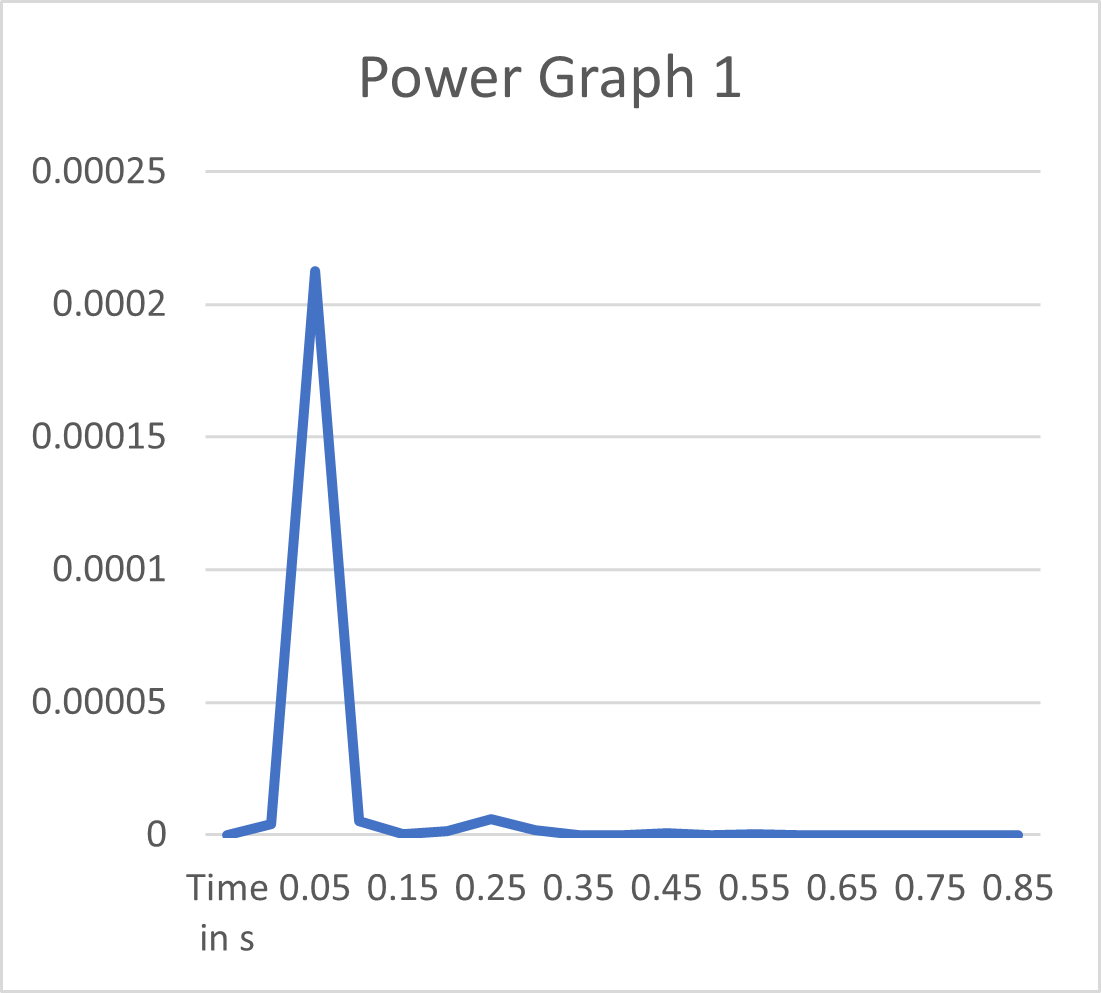
\includegraphics[width=\textwidth]{./Figure_14.png}
    \captionof{figure}{Power Graph 1}
    \label{fig:Power Graph 1}
\end{minipage}
\begin{minipage}{0.5\textwidth}
    \center
        \begin{tabular}{|c|c|}
            \hline
            Time in s & Power in P\\
            \hline
            0 & 4.85128E-08\\
            \hline
            0.05 & 2.43596E-08\\
            \hline
            0.1	& 1.64766E-08\\
            \hline
            0.15 & 1.15905E-05\\
            \hline
            0.2	& 0.000212553\\
            \hline
            0.25 & 4.17617E-06\\
            \hline
            0.3	& 3.9934E-08\\
            \hline
            0.35 & 6.97043E-08\\
            \hline
            0.4	& 1.11219E-06\\
            \hline
            0.45 & 5.00019E-06\\
            \hline
            0.5	& 7.36085E-06\\
            \hline
            0.55 & 3.27149E-06\\
            \hline
            0.6	& 3.66436E-07\\
            \hline
            0.65 & 8.51064E-10\\
            \hline
            0.7	& 8.44468E-09\\
            \hline
            0.75 & 1.58572E-07\\
            \hline
            0.8	& 1.31917E-07\\
            \hline
            0.85 & 8.09043E-08\\
            \hline
            0.9	& 5.17787E-08\\
            \hline
            0.95 & 6.20426E-09\\
            \hline
            1 & 1.64766E-08\\
            \hline
            1.05 & 5.86298E-08\\
            \hline
            1.1	& 3.70723E-08\\
            \hline
            1.15 & 9.83511E-08\\
            \hline
            1.2	& 1.84021E-08\\
            \hline
        \end{tabular}
        \captionof{table}{Values of Power Graph 2}
        \label{Tab:Values of Power Graph 2}
\end{minipage}
\begin{minipage}{0.5\textwidth}
    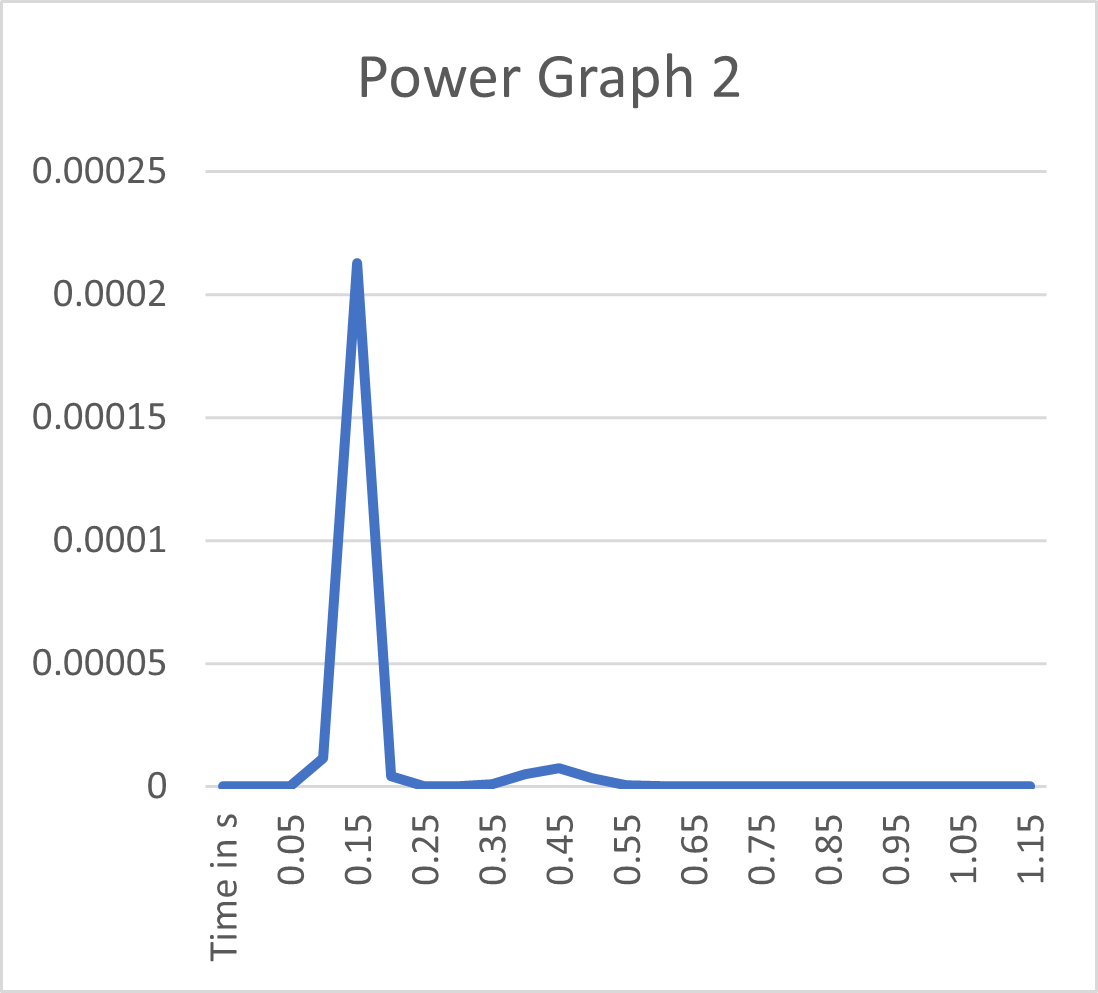
\includegraphics[width=\textwidth]{./Figure_15.png}
    \captionof{figure}{Power Graph 2}
    \label{fig:Power Graph 2}
\end{minipage}
\begin{minipage}{0.5\textwidth}
    \center
        \begin{tabular}{|c|c|}
            \hline
            Time in s & Power in W\\
            \hline
            0 & 1.42726E-07\\
            \hline
            0.05 & 6.22149E-08\\
            \hline
            0.1	& 3.16681E-08\\
            \hline
            0.15 & 2.0434E-08\\
            \hline
            0.2	& 7.0942E-06\\
            \hline
            0.25 & 0.000212553\\
            \hline
            0.3	& 1.6944E-05\\
            \hline
            0.35 & 7.43151E-07\\
            \hline
            0.4	& 7.68085E-08\\
            \hline
            0.45 & 8.17872E-07\\
            \hline
            0.5	& 2.77968E-06\\
            \hline
            0.55 & 4.14642E-06\\
            \hline
            0.6	& 1.60673E-06\\
            \hline
            0.65 & 2.45957E-09\\
            \hline
            0.7	& 3.16681E-08\\
            \hline
            0.75 & 1.64766E-08\\
            \hline
            0.8	& 2.12766E-10\\
            \hline
        \end{tabular}
        \captionof{table}{Values of Power Graph 3}
        \label{Tab:Values of Power Graph 3}
\end{minipage}
\begin{minipage}{0.5\textwidth}
    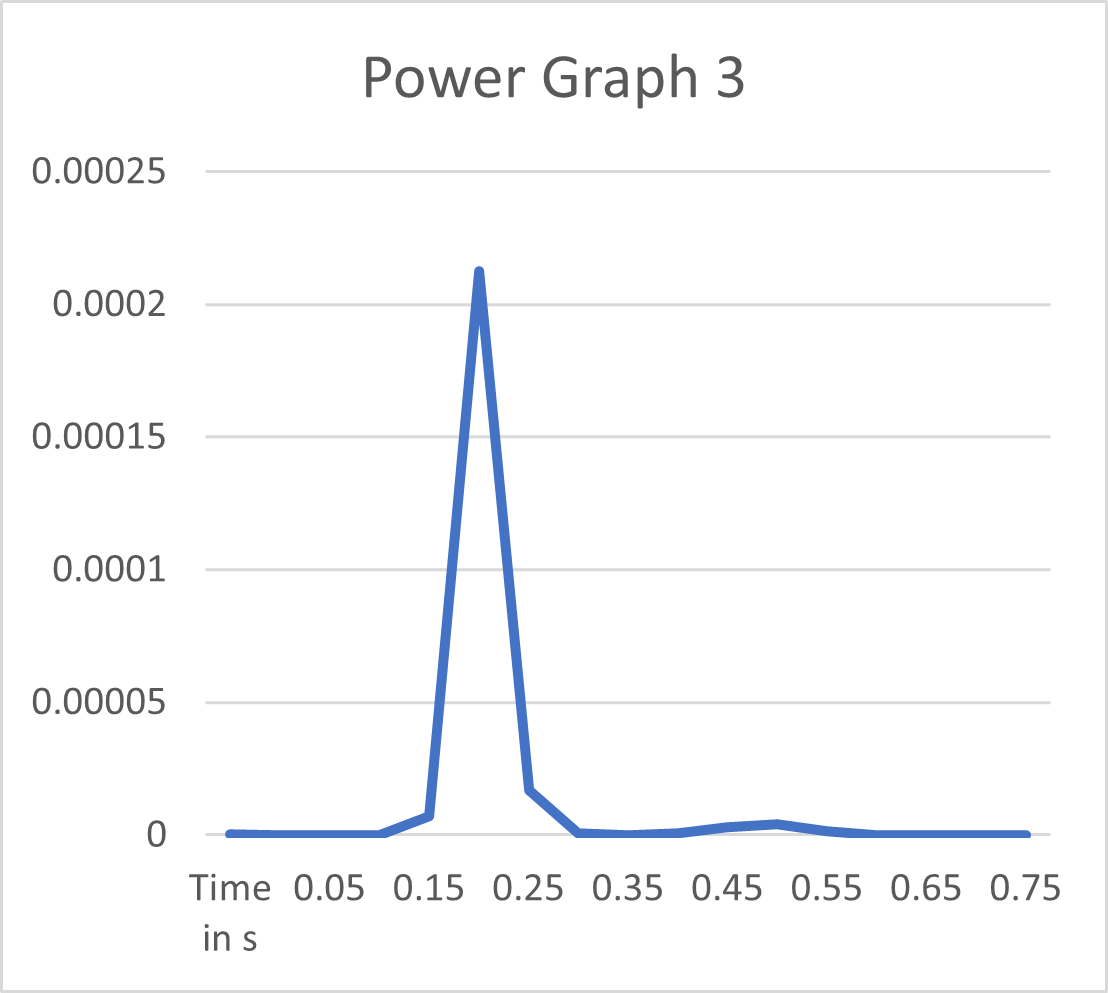
\includegraphics[width=\textwidth]{./Figure_16.png}
    \captionof{figure}{Power Graph 3}
    \label{fig:Power Graph 3}
\end{minipage}

\vspace{0.5cm}

From the table and graphs above, one can see that power produced by the piezoelectric elements varies between $2.18 \cdot 10^{-10} \pm 0.53 \cdot 10^{-10}$ W and $2130000 \cdot 10^{-10} \pm 107000 \cdot 10^{-10}$ W with a discrepancy of $8.53 \pm 4.72\%$.